\chapter{PROTÓTIPO}
\label{chap:prototipos}

Neste capítulo, apresentam-se os três protótipos experimentais desenvolvidos para viabilizar o fatiamento de rede (\textit{network slicing}) e o provisionamento de Qualidade de Serviço (QoS) em redes cientes de caminho por meio do sistema de numeração de resíduos (RNS, do inglês \textit{Residue Number System}). A construção segue uma estratégia incremental de validação arquitetural, cobrindo distintos níveis de fidelidade de hardware, flexibilidade de programação e desempenho de encaminhamento:

\begin{enumerate}
    \item \textbf{Protótipo 1 -- Hardware programável (Tofino/freeRtr):} infraestrutura física interestadual com enlaces de 10~Gbps e comutadores baseados no circuito integrado Intel Tofino\textregistered, operando sob o \textit{framework} de controle freeRtr\footnote{\url{http://www.freertr.org/}}, concebida para validar o fatiamento estritamente por meio da seleção explícita de caminhos fim a fim no PolKA original;
    \item \textbf{Protótipo 2 -- Ambiente comportamental P4 (BMv2/Mininet):} implementação em software voltada à validação das extensões da arquitetura \nome, elevando a granularidade do fatiamento ao codificar simultaneamente a rota e a fila de escalonamento em um único rótulo, acoplada a um \textit{Traffic Manager} customizado em C++ com escalonamento ponderado (\textit{Weighted Deficit Round-Robin} -- WDRR);
    \item \textbf{Protótipo 3 -- Infraestrutura virtualizada em contêineres (Containerlab/eBPF):} topologia orquestrada via Containerlab sobre contêineres Ubuntu 24.04, empregando programas eBPF/XDP no plano de dados para realizar a classificação, o encapsulamento e o encaminhamento em alta velocidade integrados ao subsistema nativo de controle de tráfego (\texttt{tc}) do \textit{kernel} Linux.
\end{enumerate}

A coexistência dessas três frentes de prototipação fundamenta-se nas características e limitações de cada ecossistema. As operações aritméticas de plano de dados introduzidas pelo \nome\ preservam a mesma base algébrica do PolKA tradicional, cuja viabilidade em taxa de linha já foi demonstrada em comutadores Intel Tofino por \textcite{dominicini2021}. Contudo, como o plano de controle freeRtr ainda não contempla nativamente as extensões de cabeçalho e o fatiamento de bits (\textit{bit-slicing}) para seleção de fila do \nome, desenvolveu-se o segundo protótipo no ambiente comportamental P4/BMv2 sobre o emulador Mininet, seguido pela implementação nativa em eBPF/XDP no Containerlab para avaliação em ambiente baseado em sistema operacional Linux.

Nos protótipos do \nome, a borda de ingresso classifica o tráfego entrante a partir de identificadores do cabeçalho (como o campo DSCP do modelo DiffServ ou demais metadados de fluxo) para mapear rotas e classes de serviço em um único rótulo \routeID\ de 20~bytes (dimensionado para um diâmetro máximo de 10 saltos com polinômios geradores de 16~bits). No núcleo, a decodificação sem estado explora primitivas nativas de CRC-16 (em P4) ou cálculo polinomial otimizado em eBPF/XDP para extrair o identificador da porta física de saída (\portID) e o identificador da fila de serviço (\qID\ de 3~bits, endereçando até 8 filas por interface).

Nas seções seguintes, detalham-se a topologia, os componentes de software e hardware, a pilha de protocolos e a parametrização de filas de cada protótipo desenvolvido.

% ==============================================================================
\section{Protótipo 1 -- PolKA Original em Hardware Programável (Tofino/freeRtr)}
\label{sec:prototipo_porvir}

O primeiro protótipo foi implantado sobre a infraestrutura experimental nacional do projeto PORVIR \cite{Nogueira2025}, cuja topologia física interconecta quatro pontos de presença interestaduais --- Vitória (VIX), Belo Horizonte (MG), Rio de Janeiro (RJ) e São Paulo (SP) --- por meio de enlaces ópticos de 10~Gbps e comutadores programáveis baseados em ASIC Intel Tofino\textregistered, ilustrados na Figura~\ref{fig:porvir_topo}.

\begin{figure}[htbp]
    \centering
    \captionsetup{justification=centering}
    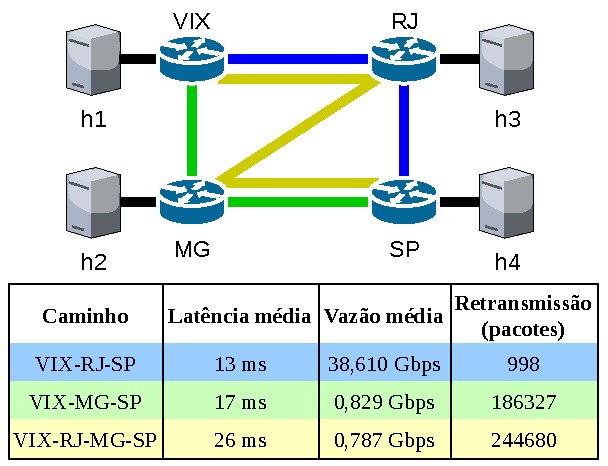
\includegraphics[width=0.65\linewidth]{figuras/Porvir - Tabela e Topo.pdf}
    \caption{Topologia interestadual do testbed nacional PORVIR utilizada no Protótipo 1.}
    \label{fig:porvir_topo}
\end{figure}

Nesse ambiente, o plano de controle é gerenciado pelo \textit{framework} freeRtr, responsável pela descoberta da topologia, pela atribuição dos identificadores polinomiais (\nodeIDs) a cada comutador de núcleo e pelo cálculo dos rótulos de roteamento na origem via Teorema Chinês dos Restos (CRT). Para possibilitar o isolamento de tráfego por meio da seleção explícita de caminhos fim a fim, foram provisionados três túneis PolKA distintos entre as bordas de Vitória e São Paulo:
\begin{itemize}
    \item \textbf{Caminho principal (VIX--RJ--SP):} rota de menor número de saltos e maior capacidade nominal, destinada às fatias de maior prioridade;
    \item \textbf{Caminho alternativo 1 (VIX--MG--SP):} rota intermediária utilizada para o desvio de fluxos concorrentes;
    \item \textbf{Caminho alternativo 2 (VIX--RJ--MG--SP):} rota secundária de maior comprimento, empregada para acomodar fluxos de menor precedência sob condições de competição no enlace principal.
\end{itemize}

A reconfiguração dinâmica das fatias nesse protótipo ocorre exclusivamente nos comutadores de borda, onde o plano de controle atualiza a associação entre o fluxo ingressante e o rótulo PolKA correspondente ao túnel de destino, redirecionando o tráfego sem alterar regras nos nós intermediários do núcleo.

% ==============================================================================
\section{Protótipo 2 -- SPolKA em Plano de Dados P4 (BMv2/Mininet)}
\label{sec:prototipo_bmv2}

Para validar o fatiamento conjunto de rotas explícitas e políticas de enfileiramento do \nome, desenvolveu-se o segundo protótipo no emulador de redes Mininet utilizando comutadores programáveis baseados na arquitetura comportamental BMv2 (\textit{Behavioral Model version 2}). A topologia experimental adotada, apresentada na Figura~\ref{fig:topologia_polka}, é composta por comutadores de borda (\texttt{e1} a \texttt{e6}), comutadores de núcleo (\texttt{s1} a \texttt{s4}, correspondentes aos nós $C_2$ a $C_5$ na representação lógica) e pares de \textit{hosts} geradores e receptores de tráfego ($H_1$--$S_1$ a $H_5$--$S_5$), interconectados por enlaces com capacidade configurada em 10~Mbps.

\begin{figure}[htbp]
    \centering
    \captionsetup{justification=centering}
    \fbox{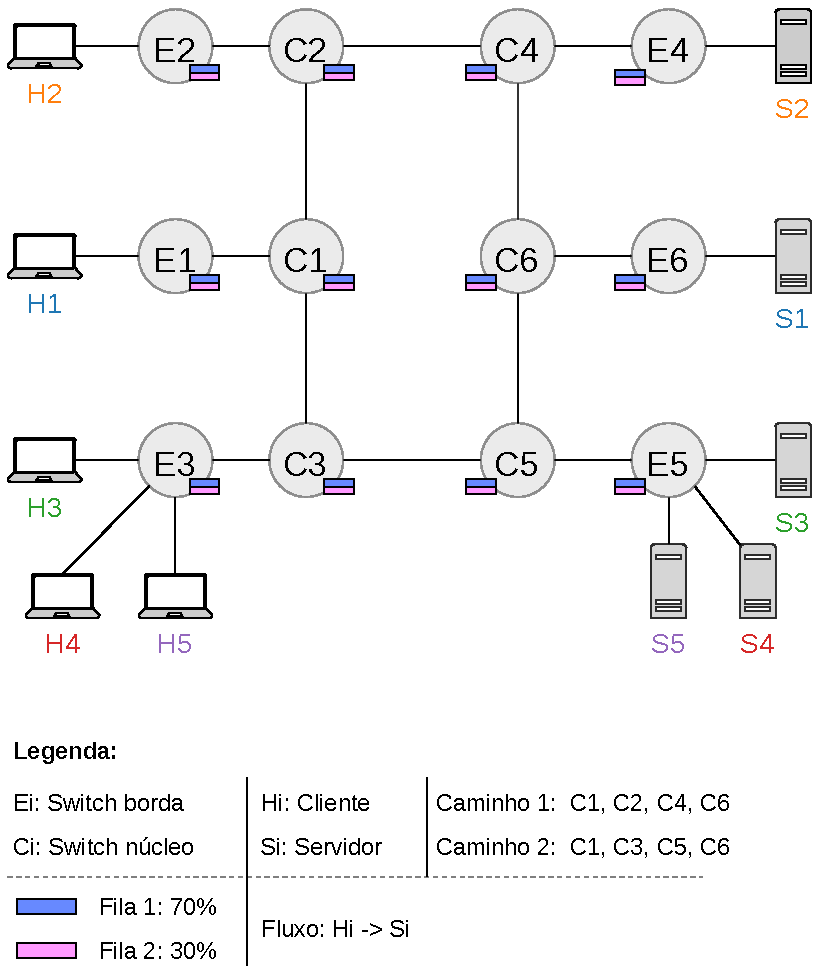
\includegraphics[width=0.75\linewidth]{figuras/topologia - SBRC WPEIF 2026_v4.pdf}}
    \caption{Topologia de rede emulada em Mininet/BMv2 para o Protótipo 2.}
    \label{fig:topologia_polka}
\end{figure}

Diferentemente do Protótipo 3 --- que classifica os pacotes com base no campo DSCP ---, no Protótipo 2 a identificação e o mapeamento das fatias na borda de ingresso são realizados a partir do **endereço IPv4 de origem** (\texttt{hdr.ipv4.srcAddr}) do fluxo entrante, demonstrando a flexibilidade do \nome\ em operar sobre distintos critérios de classificação do cabeçalho. A arquitetura interna do ambiente emulado divide-se em três componentes principais:

\begin{enumerate}
    \item \textbf{Plano de Controle e Síntese Polinomial:} 
    Um controlador centralizado implementado em Python calcula os rótulos \routeID\ de 160~bits (20~bytes, dimensionados para um diâmetro máximo de 10~saltos com polinômios geradores de grau 16) por meio da aplicação do Teorema Chinês dos Restos (CRT) polinomial sobre $GF(2)$. Em tempo de execução, o controlador povoa dinamicamente as tabelas de fluxo exclusivamente nos comutadores de borda, associando o endereço IPv4 de origem de cada fluxo ao respectivo \routeID\ codificado com a rota e a fila de serviço desejada.
    \item \textbf{Pipeline Programável em $\text{P4}_{16}$:} 
    Nos nós de borda, tabelas de correspondência exata sobre o endereço IPv4 de origem acionam a inserção do cabeçalho \nome\ (\textit{EtherType} \texttt{0x1234}) contendo o \routeID\ de 160~bits na entrada do domínio e sua remoção na borda de egresso antes da entrega ao \textit{host} de destino. Nos nós de núcleo, cada comutador executa a decodificação aritmética sem estado (\texttt{srcRoute\_nhop()}, Quadro~\ref{quad:codigo_controle}), empregando a primitiva de \textit{hash} CRC-16 customizado e o fatiamento de bits (\textit{bit-slicing}) para extrair simultaneamente a porta física de saída (\portID) e o identificador da fila (\qID).
    \item \textbf{Gerenciador de Tráfego (Traffic Manager) em C++:} 
    Como o escalonador nativo do BMv2 opera estritamente por prioridade fixa --- sujeitando filas de menor precedência à inanição (\textit{starvation}) ---, modificou-se o alvo \texttt{simple\_switch} do BMv2 para integrar um módulo externo (\textit{software extern}) em C++ baseado em \textcite{Elbediwy2025}, acoplado ao final do pipeline de \textit{Ingress}. O escalonador implementa o algoritmo \textit{Weighted Deficit Round-Robin} (WDRR) aliado a um buffer de pacotes (\texttt{TM\_buffer\_WDRR}) e a um conformador de taxa (\textit{token bucket shaper}) de 10~Mbps por interface.
\end{enumerate}

Para os testes de isolamento e migração de políticas de QoS conduzidos neste ambiente, cada interface de egresso dos roteadores de núcleo foi parametrizada com duas filas de serviço distintas no escalonador WDRR:
\begin{itemize}
    \item \textbf{Fila 1 (\texttt{qID = 001}):} fila prioritária com reserva garantida de \textbf{70\%} da largura de banda do enlace;
    \item \textbf{Fila 2 (\texttt{qID = 010}):} fila secundária com reserva garantida de \textbf{30\%} da largura de banda remanescente, capaz de aproveitar a capacidade ociosa da Fila 1 em períodos sem tráfego prioritário graças à natureza conservadora de trabalho (\textit{work-conserving}) do WDRR.
\end{itemize}
% ==============================================================================
\section{Protótipo 3 -- SPolKA em eBPF/XDP sobre Contêineres (Containerlab)}
\label{sec:prototipo_containerlab}

O terceiro protótipo foi concebido para validar a portabilidade e o desempenho do \nome\ diretamente no subsistema de rede do \textit{kernel} Linux em enlaces de 1~Gbps, sem dependência de simuladores comportamentais. A infraestrutura experimental é orquestrada via \textit{Containerlab} sobre 14 nós baseados em contêineres Ubuntu 24.04 LTS, seguindo a topologia apresentada na Figura~\ref{fig:topologia_ebpf}.

\begin{figure}[htbp]
    \centering
    \captionsetup{justification=centering}
    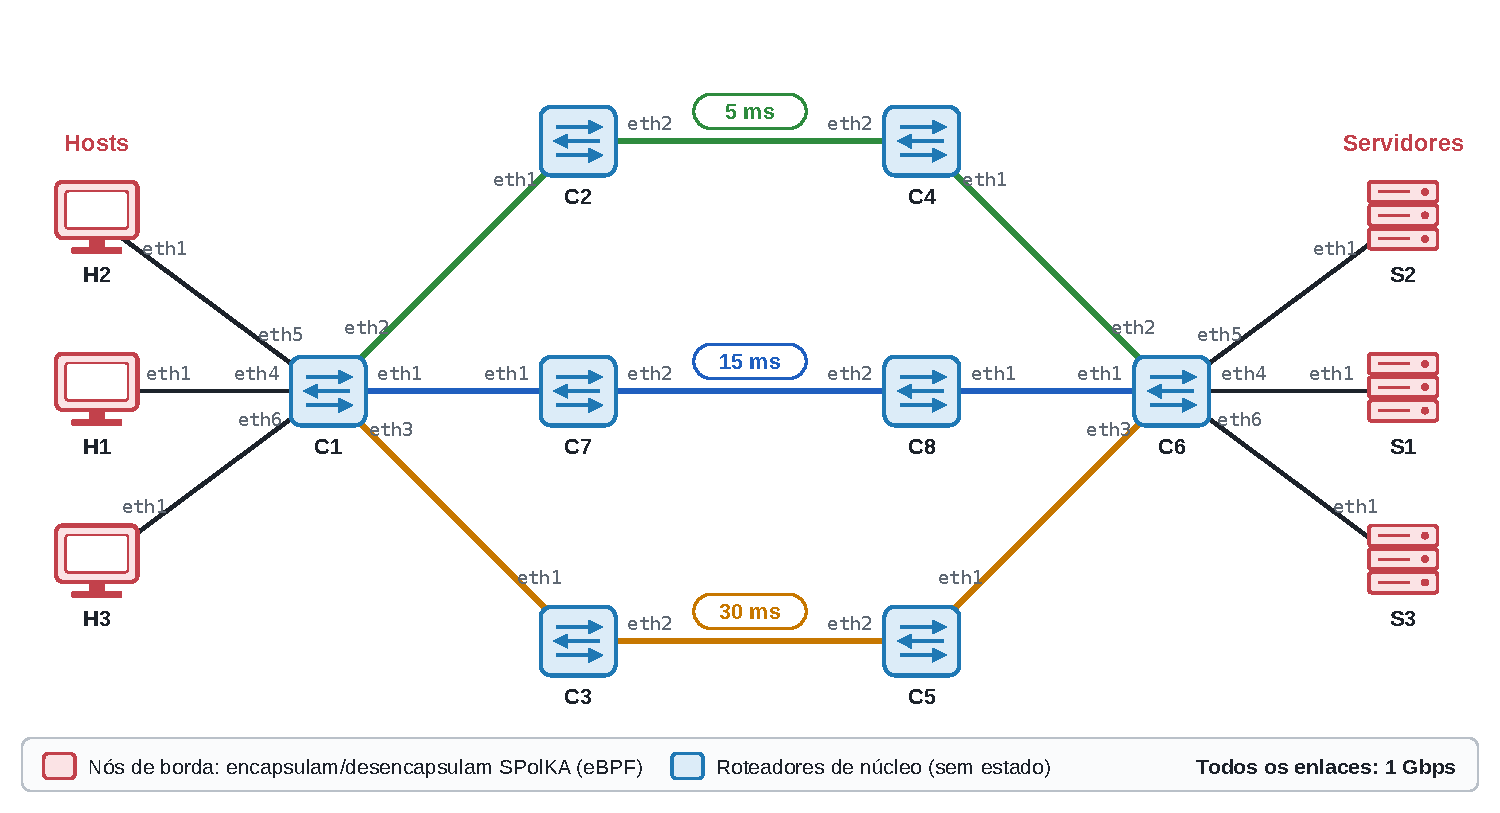
\includegraphics[width=0.85\linewidth]{figuras/fig_topologia_ebpf.pdf}
    \caption{Topologia de rede virtualizada em Containerlab/eBPF para o Protótipo 3.}
    \label{fig:topologia_ebpf}
\end{figure}

Conforme ilustrado na Figura~\ref{fig:topologia_ebpf}, a planta física interconecta três \textit{hosts} geradores ($H_1$, $H_2$ e $H_3$, na sub-rede \texttt{10.0.0.0/24}) e três servidores receptores ($S_1$, $S_2$ e $S_3$, na sub-rede \texttt{10.0.1.0/24}) via enlaces virtuais (\textit{veth}) de \textbf{1~Gbps}. Os próprios nós terminais ($H_1$--$H_3$ e $S_1$--$S_3$) atuam como \textbf{nós de borda} na interface \texttt{eth1}, enquanto os oito roteadores intermediários ($C_1$ a $C_8$) compõem o \textbf{núcleo sem estado} (\textit{stateless}), formando três caminhos disjuntos entre $C_1$ e $C_6$ com perfis distintos de latência de ida e volta (RTT):
\begin{itemize}
    \item \textbf{Caminho 1 ($C_1 \rightarrow C_2 \rightarrow C_4 \rightarrow C_6$):} rota de baixa latência com RTT configurado em \textbf{5~ms};
    \item \textbf{Caminho 2 ($C_1 \rightarrow C_7 \rightarrow C_8 \rightarrow C_6$):} rota de latência moderada com RTT configurado em \textbf{15~ms};
    \item \textbf{Caminho 3 ($C_1 \rightarrow C_3 \rightarrow C_5 \rightarrow C_6$):} rota de maior latência com RTT configurado em \textbf{30~ms}.
\end{itemize}

Para acomodar o cabeçalho compacto do \nome\ --- dimensionado neste protótipo em \textbf{8~bytes} (\textit{EtherType} \texttt{0x1234}) --- dentro do quadro Ethernet padrão de 1500~bytes sem fragmentação, as interfaces \texttt{eth1} das bordas são configuradas com MTU de 1492~bytes e ajuste automático de MSS TCP para 1420~bytes via \texttt{iptables}. Diferentemente do Protótipo 2, que requer um módulo externo em C++ no BMv2, o plano de dados em Linux divide-se em três programas eBPF compilados em C e fixados no sistema de arquivos BPF (\texttt{/sys/fs/bpf}):

\begin{enumerate}
    \item \textbf{Encapsulamento na Borda de Egresso (\texttt{spolka\_edge\_encap.c}, Apêndice~\ref{apendice:encap}):} Anexado ao gancho \texttt{TC egress} da interface \texttt{eth1} das bordas, intercepta pacotes IPv4 e realiza uma busca por correspondência de prefixo mais longo em um mapa LPM Trie (\texttt{BPF\_MAP\_TYPE\_LPM\_TRIE}, denominado \texttt{tabela\_encap}). A chave de busca combina o endereço IPv4 de destino (32~bits) e o campo DSCP mascarado (8~bits): entradas específicas de 40~bits associam uma classe de serviço a um \routeID\ dedicado, enquanto entradas de 32~bits atuam como rota padrão por destino. Identificado o fluxo, o programa insere os 8~bytes do cabeçalho \nome\ por meio da primitiva \texttt{bpf\_skb\_change\_head()}, preservando os metadados de checksum e segmentação (GSO) da pilha TCP/IP.
    \item \textbf{Encaminhamento e Classificação de Fila no Núcleo (\texttt{spolka\_core.c}, Apêndice~\ref{apendice:core}):} Anexado ao gancho \texttt{TC ingress} (\texttt{clsact}) de cada interface de dados (\texttt{eth1} a \texttt{eth6}) dos roteadores $C_1$ a $C_8$, aos quais são atribuídos polinômios irredutíveis únicos de grau 6 (\texttt{0x43} a \texttt{0x73}). Ao receber um quadro com \textit{EtherType} \texttt{0x1234}, o programa executa a divisão polinomial em $GF(2)$ diretamente em registradores de 32~bits (\texttt{poly\_mod}), extrai os 3~bits menos significativos referentes à fila (\texttt{queue\_id}) e os bits superiores referentes à porta lógica de saída (\texttt{logical\_port}), traduzindo-a para o índice de interface do \textit{kernel} via \texttt{mapa\_portas}. Em seguida, grava a fila selecionada nos metadados do pacote (\texttt{skb->priority = 0x00010000 | queue\_id}) e encaminha o quadro diretamente à fila de saída da porta de destino via \texttt{bpf\_redirect()}.
    \item \textbf{Desencapsulamento na Borda de Ingresso (\texttt{spolka\_edge\_decap.c}, Apêndice~\ref{apendice:decap}):} Anexado ao gancho \textbf{XDP nativo} (\textit{eXpress Data Path}) da interface \texttt{eth1} das bordas receptoras, remove os 8~bytes do rótulo \nome\ por meio da função \texttt{bpf\_xdp\_adjust\_head()}, restaura o \textit{EtherType} para IPv4 (\texttt{0x0800}) e entrega o pacote nativo à pilha de rede do contêiner (\texttt{XDP\_PASS}).
\end{enumerate}

Na saída de cada interface dos roteadores de núcleo, o escalonamento das fatias é realizado pelo subsistema nativo \textit{Traffic Control} (\texttt{tc}) do \textit{kernel} Linux. A hierarquia de enfileiramento combina uma disciplina \texttt{netem} na raiz (responsável por aplicar a latência de propagação de cada caminho), um conformador \texttt{tbf} (\textit{Token Bucket Filter}) configurado para a taxa nominal de 1~Gbps e uma disciplina escalonadora \texttt{drr} (\textit{Deficit Round-Robin}, \textit{handle} \texttt{1:}) composta por sete classes isoladas (\texttt{1:1} a \texttt{1:7}) com filas \texttt{bfifo} nas folhas. O metadado \texttt{skb->priority} gravado pelo programa \texttt{spolka\_core.c} endereça diretamente a classe \texttt{1:N} correspondente sem necessidade de filtros adicionais no \texttt{tc}.

Para representar um cenário realista de fatiamento multiserviço em redes cientes de caminho, o protótipo foi parametrizado com sete classes de tráfego mapeadas via DSCP (Tabela~\ref{tab:classes_servico}) e sete filas DRR com \textit{quanta} dimensionados proporcionalmente às reservas de largura de banda sobre um MTU de 1500~bytes (Tabela~\ref{tab:filas_classe_servico}).

\begin{table}[htbp]
    \centering
    \caption{Especificação e parâmetros das classes de serviço configuradas no Protótipo 3.}
    \label{tab:classes_servico}
    \begin{tabularx}{\textwidth}{lcXccc}
        \toprule
        \textbf{Classe de Serviço} & \textbf{DSCP} & \textbf{Perfil de Tráfego} & \textbf{Taxa} & \textbf{Pacote (B)} & \textbf{Prot.} \\
        \midrule
        0: \textit{low\_latency}        & 46 (EF)   & Baixa latência     & 2,00 Mbit/s & 100  & UDP \\
        1: \textit{critical\_signaling} & 40 (CS5)  & Sinalização crítica & 0,30 Mbit/s & 250  & UDP \\
        2: \textit{high\_throughput}    & 26 (AF31) & Alta vazão         & Best-effort & 1500 & TCP \\
        3: \textit{long\_living}        & 18 (AF21) & Fluxo persistente  & Best-effort & 1500 & TCP \\
        4: \textit{short\_living}       & 10 (AF11) & Rajadas curtas     & Sondagem    & 100  & ICMP \\
        5: \textit{intent\_based}       & 12 (AF12) & Baseado em intenção & 2,00 Mbit/s & 80   & UDP \\
        6: \textit{best\_effort}        & 0 (BE)    & Melhor esforço     & Best-effort & 1500 & TCP \\
        \bottomrule
    \end{tabularx}
    \fonte{Elaborado pelo autor (2026), adaptado de \textcite{puttaswamy2025pathaware}.}
\end{table}

\begin{table}[htbp]
    \centering
    \caption{Parâmetros de configuração, reserva de vazão e \textit{quantum} DRR das filas no Linux \texttt{tc}.}
    \label{tab:filas_classe_servico}
    \begin{tabularx}{\textwidth}{cccX}
        \toprule
        \textbf{Fila (\texttt{qID})} & \textbf{Banda (\%)} & \textbf{Quantum DRR (B)} & \textbf{Classe de Serviço Associada} \\
        \midrule
        1 (\texttt{1:1}) & 5  & 3.750  & \textit{Low Latency Class} \\
        2 (\texttt{1:2}) & 5  & 3.750  & \textit{Critical Signaling / Priority Class} \\
        3 (\texttt{1:3}) & 60 & 45.000 & \textit{High Throughput Class} \\
        4 (\texttt{1:4}) & 20 & 15.000 & \textit{Long Living Class} \\
        5 (\texttt{1:5}) & 3  & 2.250  & \textit{Short Living Class} \\
        6 (\texttt{1:6}) & 5  & 3.750  & \textit{Intent Based Class} \\
        7 (\texttt{1:7}) & 2  & 1.500  & \textit{Best Effort / Default Flow Class} \\
        \bottomrule
    \end{tabularx}
    \fonte{Elaborado pelo autor (2026).}
\end{table}

Com as infraestruturas experimentais, os planos de dados e os parâmetros de enfileiramento dos três protótipos devidamente especificados, o Capítulo~\ref{chap:avaliacao} apresenta a metodologia de testes, os cenários de carga avaliados e a análise comparativa dos resultados obtidos.f